\documentclass{article}
\usepackage[haranoaji]{luatexja-preset}
\usepackage{amsmath,amssymb,amsthm,mathtools}
\usepackage{xcolor}
\usepackage[top=20mm,bottom=20mm,left=15mm,right=15mm]{geometry}
\usepackage{hyperref}
\usepackage{graphicx}
\usepackage{booktabs}
\usepackage{enumitem}
\usepackage{tcolorbox}
\tcbuselibrary{skins}
\usepackage{listings}
\usepackage{tikz}
\usetikzlibrary{shapes,arrows.meta,positioning,calc,decorations.markings,automata,fit}
\usepackage{circuitikz}
\usepackage[version=4]{mhchem}
\usepackage{pgfplots}
\pgfplotsset{compat=1.18}
\usepackage{fancyhdr}
\usepackage[absolute]{textpos}
\begin{document}
\section{包括的スモークテスト}
日本語の表示テスト。\textbf{太字}、\textit{斜体}、{\small 小}。

数式: $E = mc^2$, $\alpha + \beta = \gamma$
\[
  \int_0^\infty e^{-x^2}\,dx = \frac{\sqrt{\pi}}{2}
\]
\begin{equation}
  \sum_{n=1}^{\infty} \frac{1}{n^2} = \frac{\pi^2}{6}
\end{equation}

\begin{itemize}[leftmargin=*]
  \item リスト項目1
  \item リスト項目2
\end{itemize}

\begin{tcolorbox}[colback=blue!5,colframe=blue!40,title=テスト]
tcolorbox テスト
\end{tcolorbox}

\begin{tabular}{lcc}
\toprule
項目 & 値A & 値B \\
\midrule
テスト & 1 & 2 \\
\bottomrule
\end{tabular}

化学式: \ce{H2O}, \ce{CO2 + H2O -> H2CO3}

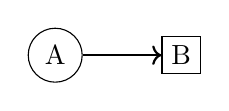
\begin{tikzpicture}
  \node[draw,circle] (a) {A};
  \node[draw,rectangle,right=of a] (b) {B};
  \draw[->,thick] (a) -- (b);
\end{tikzpicture}

\begin{circuitikz}[american]
  \draw (0,0) to[R, l=$R_1$] (2,0) to[C, l=$C_1$] (4,0);
\end{circuitikz}

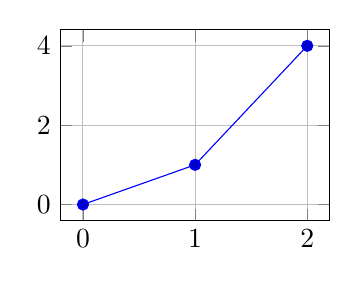
\begin{tikzpicture}
\begin{axis}[grid=major,width=5cm,height=4cm]
  \addplot coordinates {(0,0) (1,1) (2,4)};
\end{axis}
\end{tikzpicture}

\begin{lstlisting}[language=Python]
print("Hello")
\end{lstlisting}
\end{document}
